% =====================================================================
%  SchemaLens-Cassandra (TSDB / TPCx-IoT) -- Versao ajustada v1
%  Compilar no Overleaf com pdfLaTeX. Tabelas em tables/ (geradas por
%  tpcx_v1/make_tables.py a partir dos dados brutos), figuras em figs/.
% =====================================================================
\documentclass[11pt,a4paper]{article}
\usepackage[T1]{fontenc}
\usepackage[utf8]{inputenc}
\usepackage{lmodern}
\IfFileExists{brazil.ldf}{\usepackage[brazil]{babel}}{}
\usepackage[a4paper,margin=2.2cm]{geometry}
\usepackage{amsmath,amssymb}
\usepackage{graphicx}
\usepackage{booktabs,tabularx,longtable,array}
\usepackage{float}
\usepackage[font=small,labelfont=bf]{caption}
\usepackage[table]{xcolor}
\usepackage{microtype}
\usepackage{fancyhdr}
\usepackage[colorlinks=true,linkcolor=blue!50!black,urlcolor=blue!50!black]{hyperref}

\definecolor{boxbg}{RGB}{243,246,250}
\definecolor{warnbg}{RGB}{253,244,232}
\newcommand{\caixa}[2][boxbg]{\par\smallskip\noindent\colorbox{#1}{\parbox{\dimexpr\linewidth-2\fboxsep}{#2}}\par\smallskip}
\newcommand{\just}[1]{\caixa{\textbf{Justificativa.} #1}}
\newcommand{\limit}[1]{\caixa[warnbg]{\textbf{Limitação.} #1}}
\newcolumntype{Y}{>{\raggedright\arraybackslash}X}
\newcommand{\envversion}{4.1.12}
\newcommand{\envdriver}{3.30.1}
\newcommand{\envpython}{3.12.3}
\newcommand{\envcpuset}{0-3}
\newcommand{\envmem}{6}
\newcommand{\envrawreads}{7.200}
\newcommand{\envruns}{60}
\newcommand{\envdiscarded}{0}
\newcommand{\envstarted}{2026-11-17 18:09}
\newcommand{\envfinished}{2026-11-17 18:26}
\newcommand{\envothers}{5}
\newcommand{\envnoise}{6{,}1\%}
\newcommand{\envnoiseing}{3{,}4\%}
\newcommand{\envguardsamples}{60}

\makeatletter\newcommand{\tabin}[1]{\@@input #1 }\makeatother

\pagestyle{fancy}\fancyhf{}
\lhead{\small SchemaLens--Cassandra (TSDB/TPCx-IoT) --- versão ajustada v1}\rhead{\small Relatório de execução}
\cfoot{\thepage}

\title{\textbf{SchemaLens--Cassandra com o TPCx-IoT}\\[4pt]
\large Versão ajustada: nova execução da fase de medição sob o protocolo comum v1}
\author{Projeto SchemaLens / Cassandra}
\date{Execução: \envstarted--\envfinished{} UTC \quad--\quad relatório gerado em 17/11/2026}

\begin{document}
\maketitle

\begin{abstract}
\noindent Este relatório documenta a versão ajustada do experimento SchemaLens com o TPCx-IoT, segundo as correções da análise de consistência metodológica entre os benchmarks. A fase de projeto (Stages 1--8: ativação TS0/TS1/TS3, 5 candidatos, 9 coberturas admissíveis, HBench de 5) ficou congelada e foi verificada byte a byte (109 arquivos). A medição foi refeita sob o protocolo comum v1, o mesmo aplicado ao IoT-Benchmark:
\begin{itemize}
\item imagem Cassandra \envversion{} fixada por digest, em container dedicado;
\item os 9 deployments admissíveis + o baseline lógico do TPC + 2 réplicas A/A;
\item 5 repetições com reinício a frio e ordem contrabalançada, cada uma em keyspaces novos;
\item gate de flush e guarda de isolamento;
\item oráculo independente em cada leitura e auditoria integral de todos os registros após a ingestão;
\item média, p50, p95 e p99 com IC por bootstrap, piso de ruído A/A, Top-$k$, regret, Pareto em 3D, ablações e gates.
\end{itemize}
A carga do TPCx foi mantida: escrita concorrente com 2 threads de leitura de duas janelas. Ao todo foram \envrawreads{} leituras. \textbf{Resultado:} os 6 deployments que leem de uma projeção TS3 empatam entre si e são $\approx$37\% mais rápidos na leitura que os de leitura direta (TS0/TS1). O HBench contém o melhor medido, com regret 0, mas o escore do seletor não ordena a latência ($\tau=-0{,}06$): a preservação vem da salvaguarda de diversidade. O baseline lógico do TPC empata em leitura com os melhores, ingere 1,6$\times$ mais rápido que eles e ocupa metade do disco. Os 12 gates e os 11 testes negativos passaram; H1--H3 foram confirmadas e H4--H5 rejeitadas.

\end{abstract}

\tableofcontents
\newpage

\section{Resumo executivo}
\begin{enumerate}
\item \textbf{O que foi refeito.} Só a medição, sob o protocolo comum v1: imagem 4.1.12 por digest, container dedicado, os 9 deployments admissíveis + baseline + 2 réplicas A/A, 5 repetições a frio, 60 execuções aceitas (nenhuma descartada) e \envrawreads{} leituras conferidas pelo oráculo independente. Todas as execuções passaram pela auditoria integral de registros.
\item \textbf{Leitura.} Há dois grupos bem separados. Quem lê de uma projeção TS3 (partição por sensor) fica em 2,91--2,96\,ms, com 2--3 requisições CQL. Quem lê direto de TS0/TS1 fica em 4,57--5,06\,ms, com 4--6 requisições. A razão é $\approx$0,63, muito acima do piso de ruído (6,1\%). Dentro de cada grupo as diferenças são empate.
\item \textbf{Ingestão e disco.} Deployments de 1 tabela ingerem $\approx$380\,ev/s; os de 2 tabelas, $\approx$243\,ev/s (0,64$\times$). Os de 2 tabelas também ocupam $\approx$2,1$\times$ o disco. Há, portanto, um compromisso real entre leitura e escrita/armazenamento.
\item \textbf{Preservação.} O melhor medido (TS1m+TS3m, HBench \#3) e todos os empatados com ele estão no HBench: Top-3 sim, near-best sim, regret 0. O HBench retém 100\% do Pareto 2D (leitura $\times$ ingestão, critério da Etapa 9.1) e 83\% do Pareto 3D, porque fica de fora TS1h+TS3m, que empata com os demais. Em compensação, o escore do seletor não prediz a latência: $\tau=-0{,}06$, e o deployment de menor escore (TS0, o controle) é dos mais lentos. Só com $k=1$ o regret seria de 61\%.
\item \textbf{Baseline TPC.} \texttt{b\_tpcx\_logical\_raw} (uma tabela particionada por \texttt{sensor\_name}) empata em leitura com o melhor deployment do SchemaLens (razões 1,02--1,04, empate). Ele ingere 1,6$\times$ mais rápido que os deployments TS3, que precisam de 2 tabelas, e ocupa metade do disco. Nesta carga e nesta escala o baseline domina os deployments TS3 em escrita e armazenamento, sem perder em leitura.
\item \textbf{Ablações.} A regra decisiva é a de TS3: sem ela o regret sobe a 57\%. Sem TS0 o Stage 8 fica inviável, porque o controle é obrigatório. Sem TS1 o regret é de 0,2\% (empate). M1 e M3 não mudam os candidatos.
\end{enumerate}


\section{O que a análise de consistência apontou e o que foi ajustado}
\begin{longtable}{@{}p{3.6cm}p{4.8cm}p{6.6cm}@{}}
\caption{Divergências e tratamento no TPCx-IoT.}\\
\toprule \textbf{Divergência} & \textbf{Antes (Etapa 9.1)} & \textbf{Versão ajustada (v1)}\\\midrule\endhead
Crítico 2 -- versão & compose declarava \texttt{cassandra:4.1.8}; execução registrada em 4.1.12 & imagem por digest (4.1.12), container novo e dedicado, CPUs \envcpuset, \envmem\,GB; preflight confere a versão\\
Crítico 3 -- métrica/estatística & mediana do p95 de 3 repetições; sem IC nem teste & média de leitura como métrica de decisão pré-declarada; p50/p95/p99; IC bootstrap pareado pela agenda de consultas; IC $t$ de ingestão e armazenamento; piso de ruído A/A\\
Crítico 4 -- preservação & Top-$k$/regret/Pareto 2D em 3 repetições, sobre medianas de p95 & mesmos indicadores com 5 repetições, empate por ruído, Pareto em \textbf{3D} (leitura, bytes, tempo de ingestão) e também 2D, comparação com escolha aleatória\\
Repetições e ordem & 3 repetições; rotação determinística & 5 repetições com reinício a frio; permutação sorteada por par de repetições e invertida na segunda (contrabalanço)\\
Importante 10 -- ablações & nenhuma & 14 regras neutralizadas, com Stages 1--4 regenerados pelo código congelado e Stage 8 reaplicado; 5 ablações de critério\\
Importante 11 -- estado físico & \texttt{nodetool flush} só para medir armazenamento & semente gravada, \texttt{flush} e \textbf{gate} antes da fase dinâmica; guarda de isolamento na fase dinâmica; keyspace novo por execução (sem \texttt{DROP}/reset)\\
Ruído & sem controle & réplicas A/A explícitas do rank-1 (TS0) e do baseline, pré-registradas (não há pares naturais de trabalho idêntico)\\
Importantes 5, 6, 9 & próprios do benchmark & não alterados (fase de projeto congelada)\\\bottomrule
\end{longtable}

\section{Fase de projeto congelada}
\paragraph{Carga.} Duas consultas lógicas: \texttt{Q\_INGEST} (eventos TPCx com \textit{padding} de 900\,B) e \texttt{Q\_READ\_2\_WINDOWS} (leituras de duas janelas de 5\,s de um sensor, uma recente e outra histórica), no perfil analítico congelado em que o filtro é só \texttt{sensor\_name}. Os dados são sintéticos e determinísticos: 2 subestações $\times$ 3 sensores, 130 passos de semente + 500 passos medidos, ou seja, 3.780 eventos por execução. As 120 leituras usam checkpoints selados.

\paragraph{Espaço.} Ativação: TS0, TS1, TS3; M1, M3. Candidatos: \texttt{ts0\_series\_raw}, \texttt{ts1\_series\_\{3600s,60s\}} e \texttt{ts3\_sensor\_\{3600s,60s\}}. São 9 coberturas admissíveis (uma fonte canônica + no máximo uma projeção TS3); 7 estão na fronteira de Pareto analítica (5 proxies estruturais), e o HBench seleciona 5 com o controle TS0 obrigatório e diversidade de tabelas.

\paragraph{Nomes curtos.} TS0 = \texttt{ts0\_series\_raw}; TS1h/TS1m = \texttt{ts1\_series\_3600s/60s}; TS3h/TS3m = \texttt{ts3\_sensor\_3600s/60s}; BASE = \texttt{b\_tpcx\_logical\_raw} (registro lógico do TPC portado ao Cassandra, partição por \texttt{sensor\_name}; adaptação de pesquisa, não um esquema oficial). Em ``X+Y'' a leitura é roteada para a projeção (Y) quando ela existe.

\section{Execução realizada}
\begin{table}[H]\centering\small
\caption{Execução v1.}
\begin{tabularx}{\linewidth}{@{}lY@{}}\toprule
Cassandra & \envversion, nó único, RF=1, container \texttt{sl\_v1\_tpcx\_cassandra} (porta 9062), CPUs \envcpuset, \envmem\,GB\\
Cliente & Python \envpython, driver \envdriver, CPUs 8--11; \envothers{} outros containers ociosos no host\\
Variantes & 9 admissíveis + BASE + réplicas A/A de TS0 (rank 1) e de BASE = 12 por repetição\\
Por execução & keyspace novo $\rightarrow$ semente (780 eventos) $\rightarrow$ verificação $\rightarrow$ flush + gate $\rightarrow$ 10 leituras de aquecimento $\rightarrow$ fase dinâmica sob guarda (3.000 eventos, 120 leituras, 2 threads) $\rightarrow$ contagem + auditoria integral $\rightarrow$ flush + \texttt{tablestats}\\
Volume & \envruns{} execuções aceitas, \envdiscarded{} descartadas; \envrawreads{} leituras cronometradas, todas conferidas pelo oráculo; \envguardsamples{} amostras da guarda\\
\bottomrule\end{tabularx}\end{table}
\limit{A latência de leitura inclui a contenção com o writer e entre as 2 threads, que faz parte da definição da carga. A ingestão passa pela fila SQLite (\textit{outbox}) do experimento original, igual para todos. A escala é pequena e o armazenamento é medido em kB.}

\section{Resultados}
\subsection{Leitura, ingestão e armazenamento}
\begin{table}[H]\centering\small
\caption{Por variante (5 repetições). Leitura em ms com IC 95\% bootstrap da média; CQL = requisições por leitura observadas; ingestão em eventos/s (média das repetições); disco em KiB live após flush.}
\resizebox{\linewidth}{!}{\begin{tabular}{@{}llrcrrrcrr@{}}\toprule
Variante & Papel & Média & IC 95\% & p50 & p95 & p99 & CQL & ev/s & KiB\\\midrule
\tabin{tables/t_summary.tex}
\bottomrule\end{tabular}}\end{table}

\begin{figure}[H]\centering
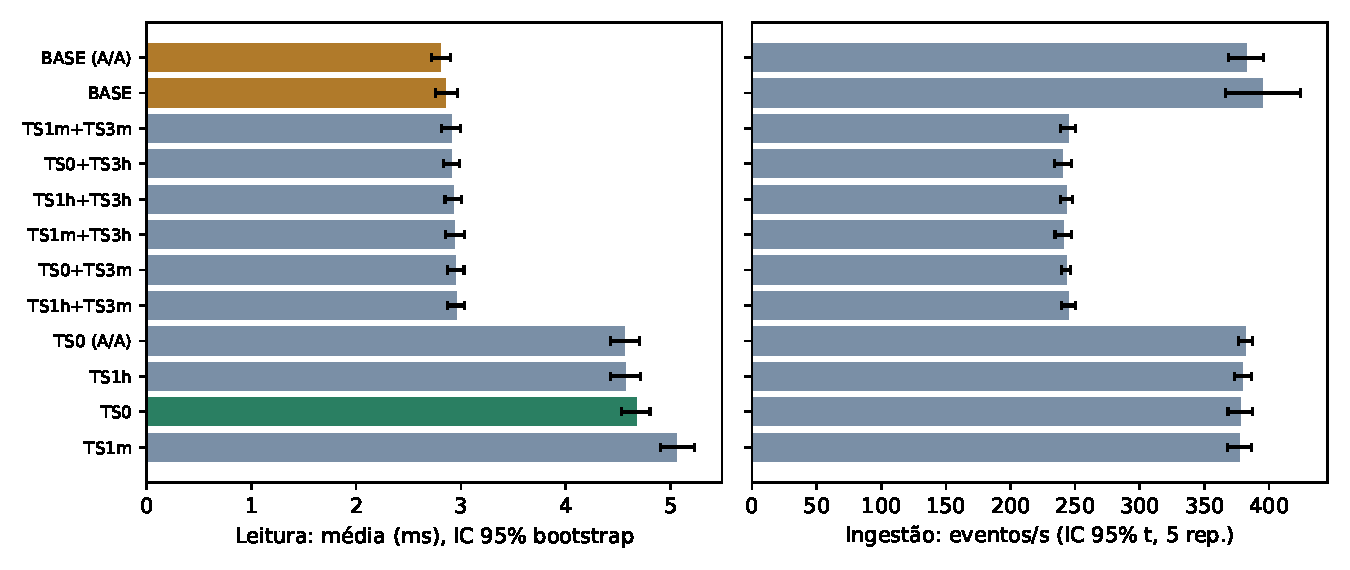
\includegraphics[width=\linewidth]{figs/fig_v1_tpcx.pdf}
\caption{Média de leitura (IC bootstrap) e taxa de ingestão (IC $t$). Verde: rank 1 do seletor; ocre: baseline TPC.}
\end{figure}
\paragraph{Leitura.} O efeito estrutural previsto pela ativação de TS3 (``projeção por sensor'') é real e grande: ler de uma partição por sensor e janela evita varrer uma partição por estação. Não importa se a fonte canônica é TS0 ou TS1, nem se o bucket é de 60\,s ou de 3600\,s (todos empatam). Os 60\,s fazem a janela cruzar o limite do bucket às vezes (3 requisições), mas sem efeito mensurável. O custo dessa leitura é escrever cada evento duas vezes.


\subsection{Piso de ruído (réplicas A/A)}
\begin{table}[H]\centering\small
\caption{Leitura: pares A/A (mesmo deployment em keyspaces diferentes, posições diferentes da ordem). Piso de ruído = \envnoise.}
\begin{tabular}{@{}lccc@{}}\toprule Par & Razão das médias & IC 95\% & q95 $|\ln r|$\\\midrule
\tabin{tables/t_noise.tex}
\bottomrule\end{tabular}\end{table}
\begin{table}[H]\centering\small
\caption{Ingestão e armazenamento nos pares A/A. Piso de ruído da ingestão = \envnoiseing.}
\begin{tabular}{@{}lcc@{}}\toprule Par & Razão ev/s & Razão bytes\\\midrule
\tabin{tables/t_noise_ing.tex}
\bottomrule\end{tabular}\end{table}

\subsection{Contrastes}
{\small\setlength{\tabcolsep}{4pt}\begin{longtable}{@{}llcclccc@{}}
\caption{Contrastes A/B (leitura: razão das médias com IC pareado; ingestão: razão de ev/s, empate abaixo do piso A/A; disco: razão de bytes).}\\
\toprule A & B & Leitura A/B & IC 95\% & Veredito & Ingestão A/B & Veredito & Disco A/B\\\midrule\endhead
\tabin{tables/t_contrasts.tex}
\bottomrule
\end{longtable}}

\subsection{Previsão estrutural (Stage 7/8 $\times$ medido)}
\begin{table}[H]\centering\small
\caption{Requisições CQL por leitura e inserts por evento: proxy do Stage 7/8 contra o observado.}
\begin{tabular}{@{}lcccc@{}}\toprule Deployment & CQL previsto & CQL observado & Inserts/evento previsto & observado\\\midrule
\tabin{tables/t_s79.tex}
\bottomrule\end{tabular}\end{table}
\paragraph{Leitura.} Os inserts por evento previstos (1 ou 2) coincidem exatamente com os observados. As requisições CQL por leitura \emph{não} coincidem em valor: o proxy foi calculado para a escala modelada no EER (10 estações, pior caso de cruzamento de bucket), e a medição usa 2 estações. Por isso a H5 pré-registrada foi rejeitada. A \emph{ordem} se preserva: TS3 (3 previsto; 2--3 observado) $<$ TS0 (20; 4) $\le$ TS1 (30; 4--6). Fica a lição para o protocolo: o proxy estrutural precisa ser recalculado na escala executada antes de ser comparado.


\subsection{Avaliação do método no espaço admissível}
\begin{table}[H]\centering\small
\caption{Indicadores de preservação (9 deployments medidos).}
\begin{tabularx}{\linewidth}{@{}lY@{}}\toprule
\tabin{tables/t_method.tex}
\bottomrule\end{tabularx}\end{table}
\paragraph{Leitura.} Em contraste com o IoT, no TPCx o escore ponderado (45/15/20/15/5, normalizado pelo controle TS0) favorece TS0, porque os proxies de armazenamento, inserts e partições penalizam as projeções. Ainda assim a seleção preservou o melhor, por causa da diversidade de tabelas: controle + uma variante de cada tabela física. Isso confirma o papel da salvaguarda de diversidade e, ao mesmo tempo, mostra que os pesos do escore não estão alinhados com a métrica de leitura. Isso é coerente com a divergência importante 5 da análise (pesos declarados, mas arbitrários).


\subsection{Ablações}
\begin{longtable}{@{}p{3.8cm}p{5.4cm}rcp{3.4cm}@{}}
\caption{Ablações de regra (Stages 1--4 regenerados com a regra neutralizada; Stage 8 reaplicado) e de critério. Regret com as medições v1.}\\
\toprule Ablação & HBench resultante & Regret & Near-best & Observação\\\midrule\endhead
\tabin{tables/t_ablation.tex}
\bottomrule
\end{longtable}
\paragraph{Leitura.} A neutralização roda de verdade o pipeline (Stages 1--3) e o Stage 4. O Stage 5 congelado exige exatamente 5 candidatos, que é um contrato do design, então o Stage 8 é reaplicado com as funções do consolidador sobre as coberturas que sobrevivem. A regra de TS3 é a única cuja ausência degrada fortemente o HBench (regret 57\%). Sem TS0 a seleção fica inviável pela política de controle obrigatório; sem esse controle, a diversidade ainda encontra o melhor. A escolha aleatória de 5 em 9 tem regret esperado de só 0,2\%, porque 6 dos 9 deployments empatam com o melhor. O espaço é pouco discriminante para regret em leitura: o compromisso relevante está na escrita.


\subsection{Comparação com a Etapa 9.1 (verification)}
\begin{table}[H]\centering\small
\caption{Etapa 9.1 (mediana de 3 repetições, sem latências brutas preservadas) $\times$ v1 (5 repetições).}
\begin{tabular}{@{}lrrrrrrr@{}}\toprule
 & \multicolumn{3}{c}{Etapa 9.1} & \multicolumn{4}{c}{v1}\\\cmidrule(lr){2-4}\cmidrule(lr){5-8}
Deployment & med. p95 & ev/s & KiB & média & p95 & ev/s & KiB\\\midrule
\tabin{tables/t_legacy.tex}
\bottomrule\end{tabular}\end{table}
\paragraph{Leitura.} A Etapa 9.1 não preservou latências brutas, então não é possível recalcular sua estatística; a comparação é de ordenação. O $\tau$ entre o p95 mediano antigo e a média v1 é 0,78. O melhor antigo (TS0+TS3h) está no grupo empatado com o melhor da v1, e as conclusões qualitativas se mantêm (TS3 lê mais rápido, 2 tabelas ingerem mais devagar). A v1 acrescenta IC, piso de ruído, Pareto 3D e o resultado do baseline, que antes aparecia só como razão de medianas. O armazenamento absoluto difere entre as duas execuções (flush em momentos diferentes da execução), mas as razões entre deployments se mantêm.


\section{Hipóteses pré-registradas}
\begin{longtable}{@{}p{0.7cm}p{5.8cm}p{1.8cm}p{6.4cm}@{}}
\toprule & Hipótese & Resultado & Evidência\\\midrule\endhead
\tabin{tables/t_hyp.tex}
\bottomrule
\end{longtable}
H4 foi rejeitada porque o HBench não contém TS1h+TS3m, que pertence ao Pareto 3D medido (empata em leitura com o melhor e não é dominado em bytes/escrita). H5 foi rejeitada por diferença de escala dos proxies (ver a seção sobre o Stage 7). As duas rejeições ficam registradas como resultado; nenhuma hipótese foi reescrita depois da medição.


\section{Aceitação}
\begin{minipage}[t]{0.5\linewidth}\centering\small
\begin{tabular}[t]{@{}lc@{}}\toprule Gate (dados brutos) & \\\midrule
\tabin{tables/t_gates.tex}
\bottomrule\end{tabular}\end{minipage}\hfill
\begin{minipage}[t]{0.48\linewidth}\centering\small
\begin{tabular}[t]{@{}lc@{}}\toprule Teste negativo & \\\midrule
\tabin{tables/t_neg.tex}
\bottomrule\end{tabular}\end{minipage}

\medskip
Os gates foram recalculados a partir de \texttt{raw\_reads.csv} e \texttt{manifest.json}: 60/60 execuções completas, oráculo em todas as leituras, auditoria integral de todos os registros físicos, 0 compactações durante as janelas, agenda de consultas idêntica (mesmo SHA-256) em todas as execuções e leituras concorrentes com a ingestão em todas. \textbf{Status: ACEITO.}


\section{O que muda nas conclusões do TPCx-IoT}
\begin{enumerate}
\item \textbf{Comparabilidade.} O TPCx-IoT passa a usar a mesma imagem, as mesmas métricas, a mesma estatística, o mesmo controle físico e os mesmos indicadores de preservação que o IoT-Benchmark.
\item \textbf{Confirmado:} a projeção TS3 por sensor reduz a latência de leitura em $\approx$37\%, ao custo de $\approx$36\% de ingestão e 2$\times$ de disco; o HBench preserva o melhor (regret 0) e o Pareto 2D.
\item \textbf{Novo e importante para o artigo:} (i) o escore do seletor não prediz a leitura ($\tau=-0{,}06$), e a preservação depende da diversidade; (ii) o baseline lógico do TPC (uma tabela por sensor) empata em leitura com o melhor deployment do SchemaLens e é melhor em escrita e disco. A restrição ``TS3 não pode ser fonte canônica'' do catálogo exclui exatamente esse desenho. É uma limitação do espaço de candidatos, não da medição.
\item \textbf{Para o artigo.} Não escrever que o SchemaLens supera o baseline TPCx. Escrever que a redução 9 $\rightarrow$ 5 preservou os melhores deployments do espaço SchemaLens e que, nesta carga, o baseline lógico é competitivo. Recomenda-se revisar a política de fonte canônica (permitir TS3 canônico quando a carga só filtra por sensor) e recalcular os proxies na escala executada.
\end{enumerate}


\section{Limitações}
\begin{itemize}
\item Esta é uma adaptação de pesquisa, não o TPCx-IoT oficial: não há IoTps, kit nem RF $\geq$ 2, e o filtro só por \texttt{sensor\_name} continua sendo uma hipótese não verificada no kit oficial.
\item A escala é pequena (3.780 eventos por execução, 6 séries), os dados são sintéticos e a latência é medida no cliente Python, incluindo a contenção com o writer.
\item Os proxies do Stage 7/8 são calculados para a escala modelada no EER, não para a escala executada; a comparação estrutural é de ordem, não de valor.
\item Modelo de custo, seletor e baseline continuam próprios do benchmark (importantes 5, 6 e 9).
\end{itemize}

\appendix
\section{Reprodução}
\begin{verbatim}
cd versao_ajustada/tpcx_iot_benchmark
./run_all.sh smoke | freeze | measure | analyze | ablation | accept
../.venv/bin/python tpcx_v1/make_tables.py --run outputs/v1_run1
./run_all.sh report
\end{verbatim}
\end{document}
